\section{Serbatoio aria compressa}
In conclusione della relazione, si procede ora all'analisi relativa al serbatoio.\\
Si definisce recipiente \emph{un alloggiamento progettato e costruito per contenere fluidi pressurizzati comprendente gli elementi annessi diretti sino al punto di accoppiamento con altre attrezzature}.
\subsection{Geometria del serbatoio da 100 lt} 
La geometria del serbatoio è costituita da un tratto cilindrico centrale e due fondi semiellittici, il cui volume complessivo di progetto deve essere pari a 100 lt.\\
Partendo da tale dato, è possibile calcolare approssimativamente i dati geometrici caratteristici attraverso la formula nota:
\begin{equation}
    V=V_{cil}+2\cdot V_{semisfera}=\frac{\pi D^2}{4}L+2\left(\frac{\pi D^3}{12}\right)=100\ lt. 
\end{equation}
Si suppone un valore del rapporto $\frac{L}{D}$ compreso tra $1,5$ e $4$, in modo tale da non essere rispettivamente troppo tozzo o troppo snello.\\ 
Scegliendo quindi un diametro $D=350\ mm$ si ottiene una lunghezza complessiva del serbatoio $L=923\ mm$. Il rapporto $\frac{L}{D}\simeq 2,6$ risulta quindi verificato.\\
Consultando il catalogo Baglioni è possibile quindi identificare il serbatoio VEC01095, idoneo al dimensionamento geometrico appena ottenuto.
\begin{figure}[h]
    \centering
    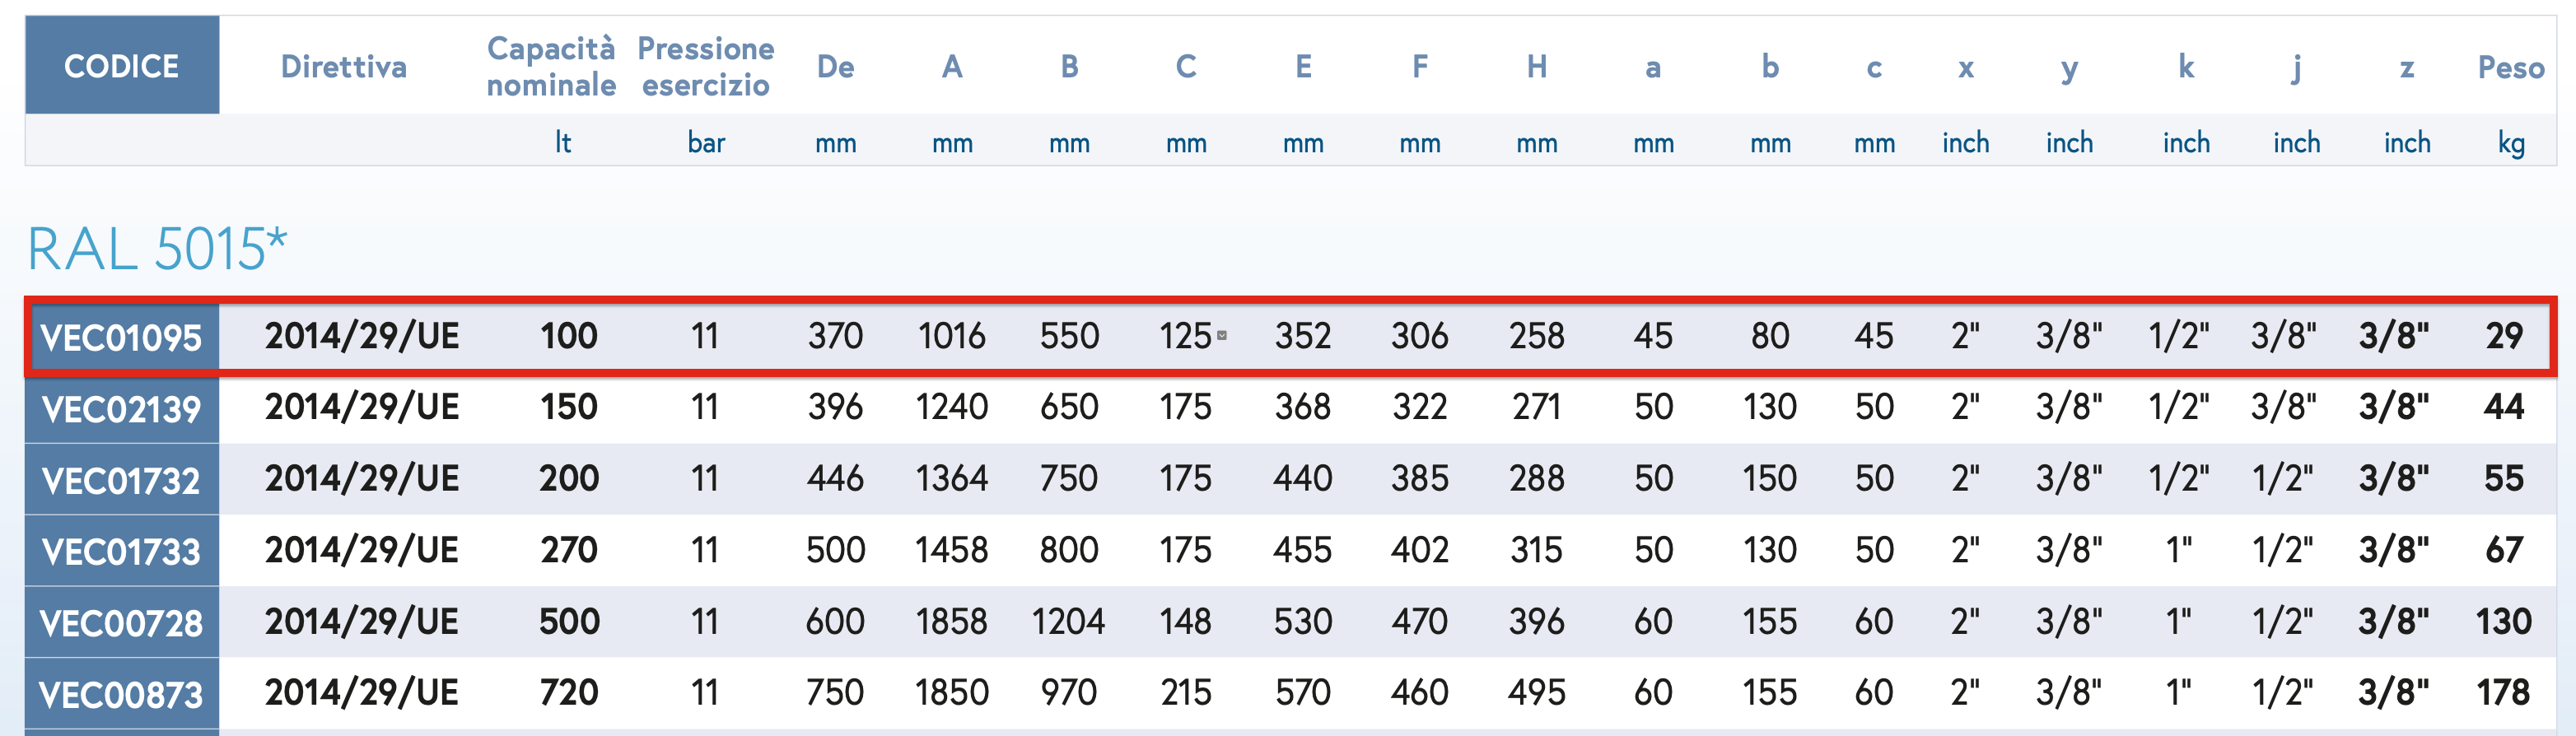
\includegraphics[scale=0.27]{Immagini/CatalogoSerbatoio1.png}
    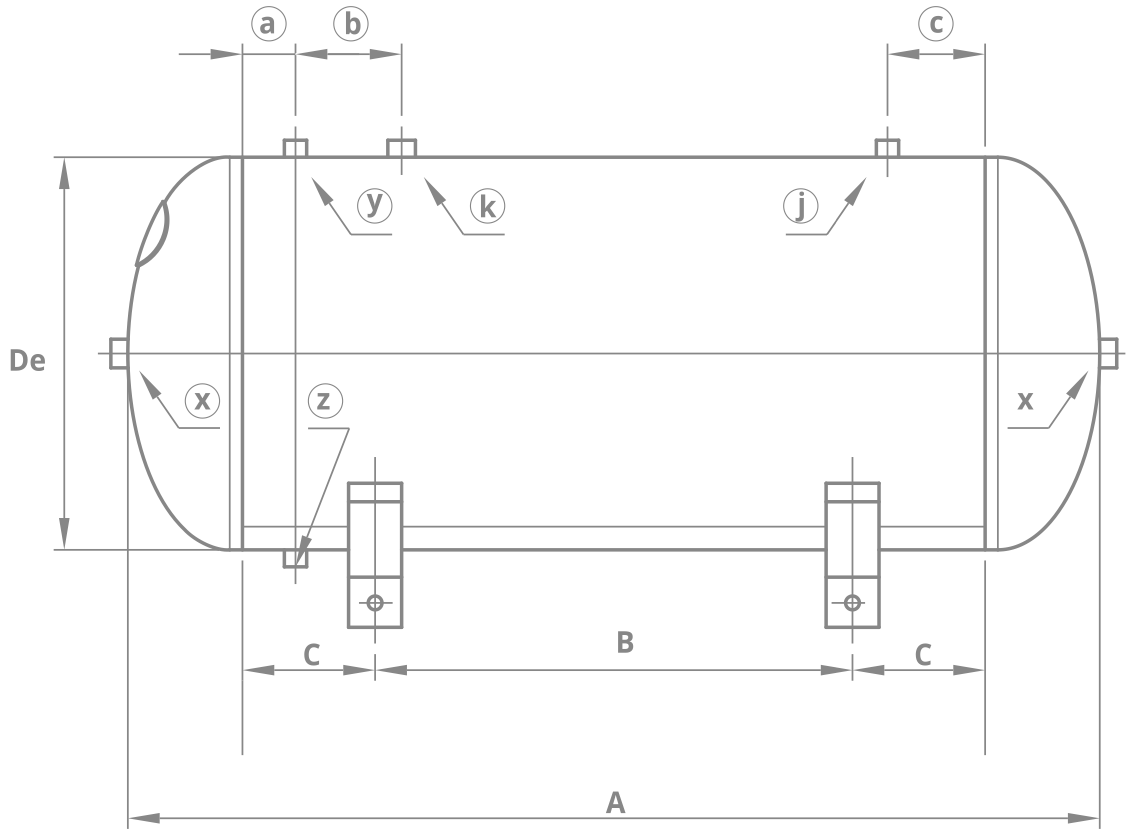
\includegraphics[scale=0.45]{Immagini/CatalogoSerbatoio2.png}
    \caption{Catalogo Baglioni SpA per serbatoi in pressione orizzontali verniciati}
    \label{fig:CatalogoSerbatoio}
\end{figure}
\newpage
\subsection{Geometria dei fondi}
I fondi del serbatoio hanno una geometria semiellittica, le cui estremità sono raccordate alla parete cilindrica centrale.\\
I parametri che definiscono tale geometria sono:
\begin{itemize}
    \item $D_e$, diametro esterno della superficie cilindrica;
    \item $H$, altezza del fondo misurata sulla superficie esterna, a partire dal piano dove ha inizio il raccordo tra parte curva e quella cilindrica;
    \item $s$, spessore di parete;
\end{itemize}
Da catalogo precedentemente considerato si ha che $H=108\ mm$ e $D_e=370\ mm$.
\begin{figure}[h]
    \centering
    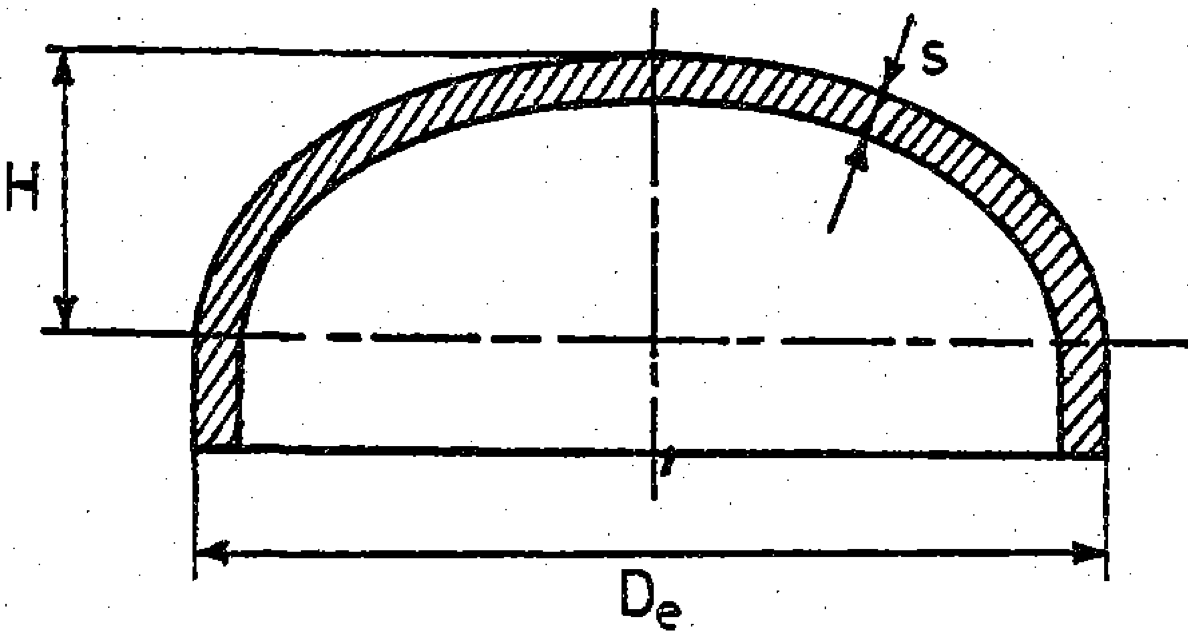
\includegraphics[scale=0.25]{Immagini/FondoSerbatoio.png}
    \caption{Geometria dei fondi del serbatoio}
    \label{fig:FondoSerbatoio}
\end{figure}
\subsection{Elementi costitutivi del piping}
Prima di analizzare e verificare il serbatoio, si procede con un focus sugli elementi caratteristici sempre presenti e necessari al funzionamento del compressore. 
\begin{figure}[h]
    \centering
    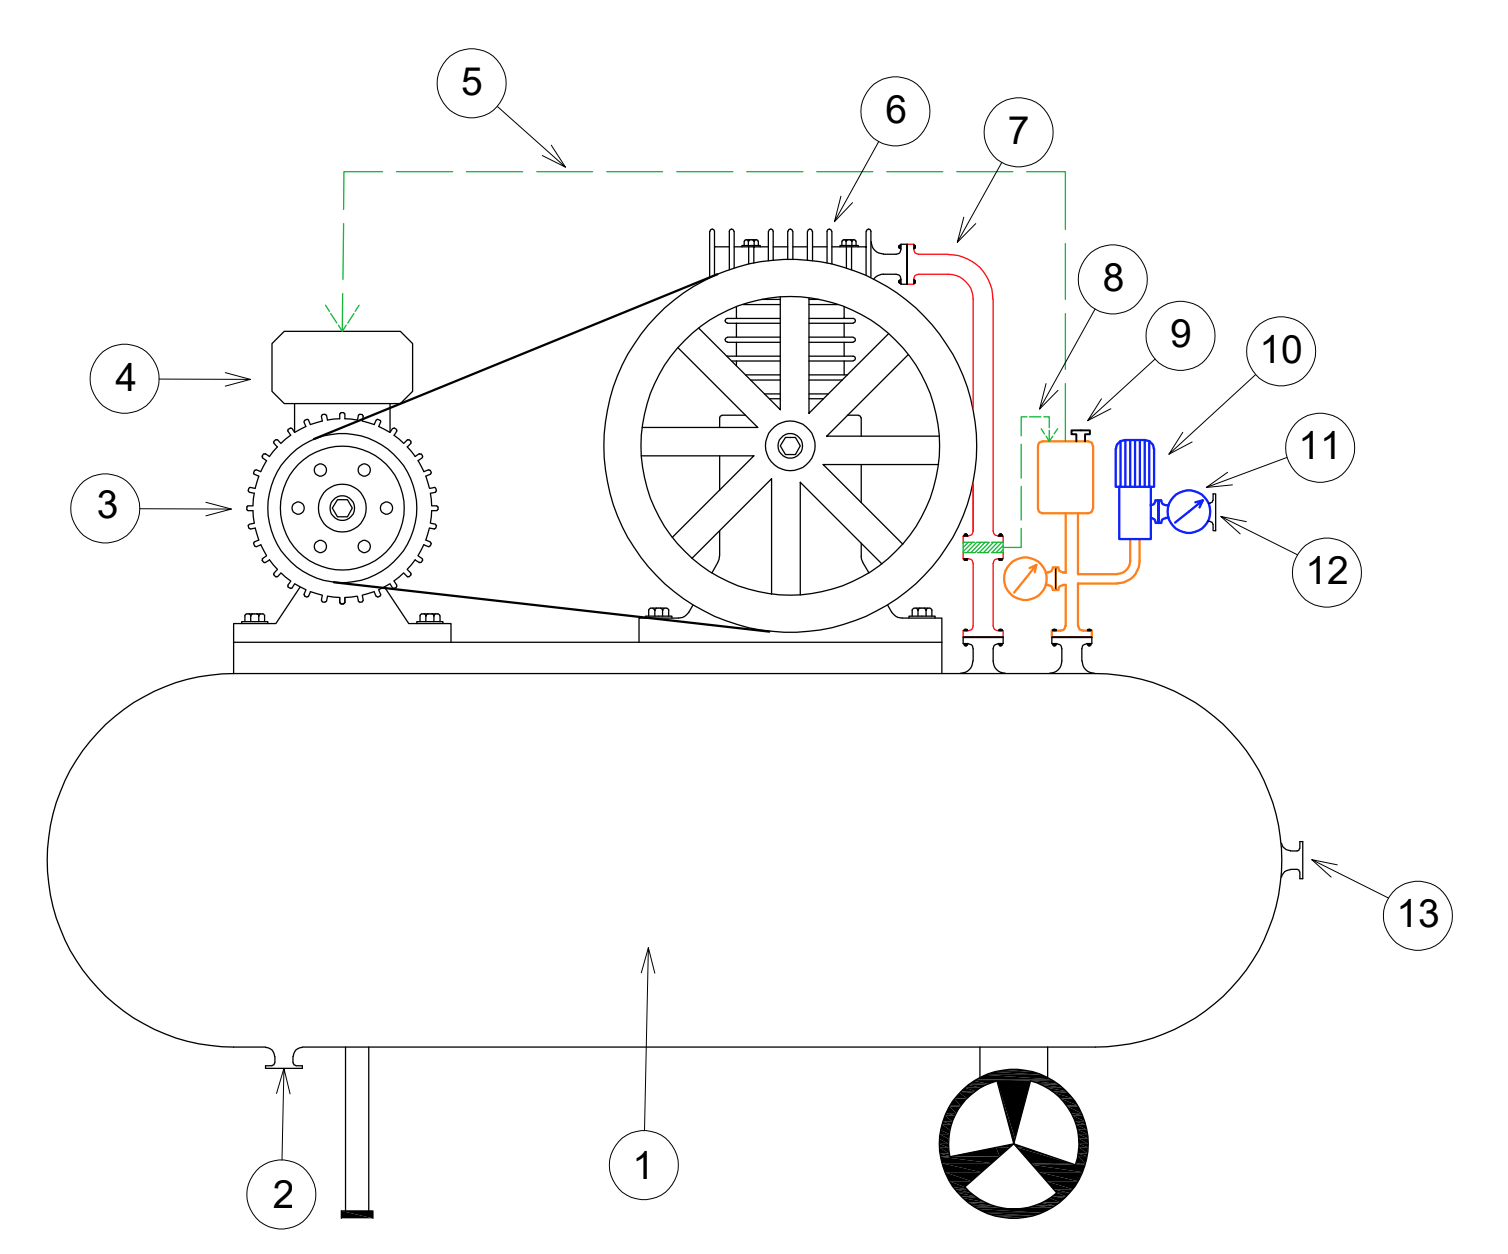
\includegraphics[scale=0.4]{Immagini/AssiemePipingCompressore.png}
    \caption{Schema costruttivo compressore FIAC}
    \label{fig:AssiemePipingCompressore}
\end{figure}
\newpage
\begin{tabular}{|l|l|l|}
\hline
    1 & Serbatoio & Elemento finalizzato allo stoccaggio del fluido pressurizzato\\
    \hline
    2 & Scarico condensa & Foro finalizzato allo scarico delle condense e olio\\
    \hline
    3 & Motore elettrico & Motore elettrico asincrono trifase a due poli\\
    \hline
    4 & Inverter & Dispositivo elettronico per il controllo del motore elettrico\\
    \hline
    5 & Pilotaggio motore & Cavo di comunicazione pressostato - inverter\\
    \hline
    6 & Compressore & Macchina finalizzata alla compressione del fluido\\
    \hline
    7 & Mandata & Tubo di mandata tra compressore e serbatoio\\
    \hline
    8 & Scarico pressostato & Linea di pressione funzionale al pressostato\\
    \hline
    9 & Pressostato & Dispositivo elettronico per il controllo della pressione\\
    \hline
    10 & Valvola RP & Valvola riduttrice di pressione \\
    \hline
    11 & Manometro & Dispositivo meccanico per la lettura delle pressioni\\
    \hline
    12 & Utenza 1 & Utenza a valle della valvola riduttrice di pressione\\
    \hline
    13 & Utenza 2 & Utenza alla massima pressione disponibile\\
    \hline
\end{tabular}
\subsection{Materiali e processi produttivi} 
\subsubsection{Materiale}
Per quanto concerne la scelta del materiale, si può fare affidamento sul D.M. 21/11/1972 \emph{Norme per la costruzione degli apparecchi in pressione}. Nel sottocapitolo \emph{Disposizioni per l'impiego di materiali nella costruzione e riparazione degli apparecchi a pressione} sono fornite indicazione riguardo la scelta dello stesso:\\
\\
\emph{Art. 8. —Nella progettazione di generatori d.i vapore, di recipienti di vapore o gas e di apparecchi a pressione in genere soggetti alle norme di cui al regio decreto 12 maggio 1927, n. 824, si deve prevedere l’impiego di materiali aventi caratteristiche chimiche o tecnologiche idonee alle condizioni di esercizio degli apparecchi medesimi, tenendo conto delle esigenze della sicurezza per l’incolumità delle persone.\\
Sono considerati rispondenti a quanto previsto nel presente articolo gli acciai al carbonio 0 legati in getti, laminati, fucinati, trafilati o simili, le ghise, il rame e sue leghe, l’alluminio e sue leghe, i1 nichel e sue leghe, il titanio ed altri materiali, purché impiegati secondo le indicazioni fornite dal1’Associazione nazionale per i1 controllo della combustione, su con- forme parere del consiglio tecnico, con la specificazione della denominazione corrente, dei valori delle caratteristiche chimiche e meccaniche, nonché dei li- miti inferiori e superiori delle temperature di impiego.\\
\\
Art. 9. —Nella costruzione di apparecchi a pressione devono essere impiegati i materiali previsti nel progetto e devono essere adottati procedimenti di lavorazione e trattamenti termici tali da non compromettere l'idoneità dei materiali stessi allo specifico uso.\\}
\\
Coerentemente con quanto riportato, la scelta del materiale è ricaduta su un acciaio al carbonio Fe360 (S235) con $R_m=360\ MPa$ e $R_s=235\ MPa$. 
\subsubsection{Processi produttivi}
La parte cilindrica centrale del serbatoio viene realizzata mediante un processo produttivo per calandratura, chiusa poi da una saldatura longitudinale.\\
Una volta realizzato il corpo cilindrico si eseguirà un processo di foratura volto alla realizzazione delle sedi per l'allacciamento delle utenze, scarico condensa e mandata. \\
I fondi semiellittici sono invece realizzati mediante un processo di imbutitura e uniti al corpo centrale nuovamente mediante saldatura.
\paragraph{Calandratura} La calandratura è un processo di produzione industriale di tipo deformazione plastica che consente di produrre o trasformare fogli di materiale o profilati metallici.\\
Le calandre utilizzate per questa lavorazione possono essere dotate di tre o quattro rulli ad assi paralleli disposti in modo tale che il foglio di lamiera, per passare tra di essi, segua una traiettoria circolare, il cui raggio di curvatura si regola agendo sulla posizione reciproca dei rulli. Si ottengono così forme coniche o cilindriche. Con apposite calandre si può ottenere la curvatura a freddo di profilati metallici.\\
\begin{figure}[h]
    \centering
    \includegraphics[scale=0.118]{Immagini/Calandratura1.png}
    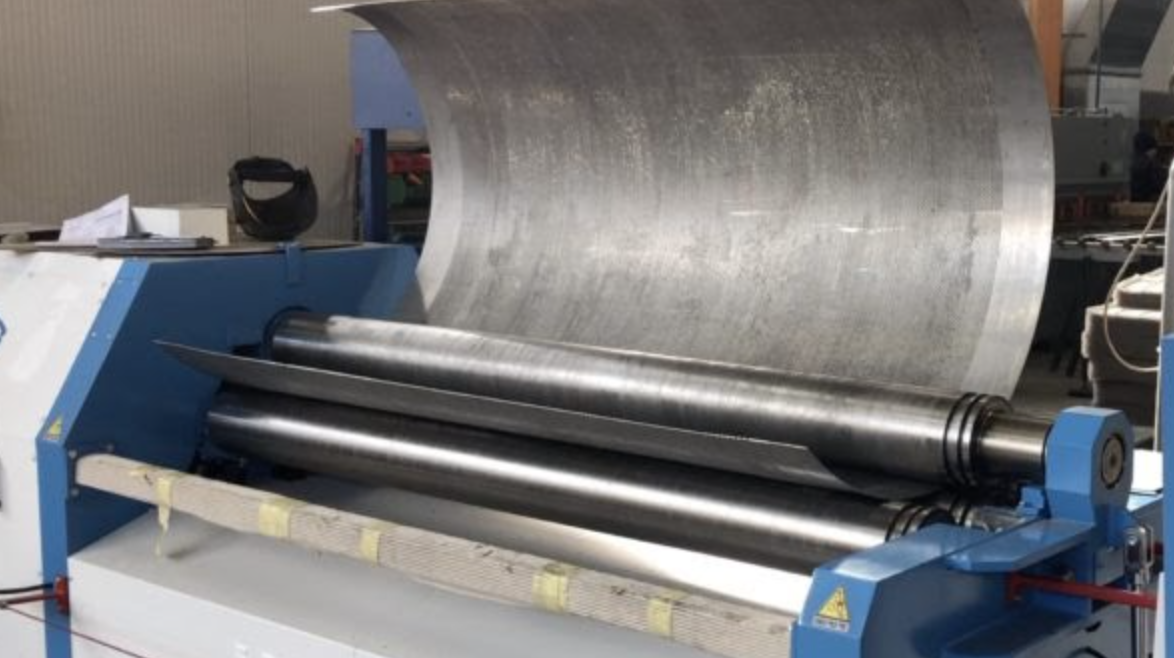
\includegraphics[scale=0.3]{Immagini/Calandratura2.png}
    \caption{Processo produttivo di calandratura}
    \label{fig:Calandratura}
\end{figure}
\paragraph{Imbutitura} L'imbutitura è un processo tecnologico attraverso il quale una lamiera viene deformata plasticamente ed assume una forma scatolare, cilindrica o a coppa.\\
Tali operazioni vengono effettuate attraverso l'uso di un punzone che spinge la lamiera, eventualmente fissata con un premilamiera, all'interno di una matrice.
\begin{figure}[h]
    \centering
    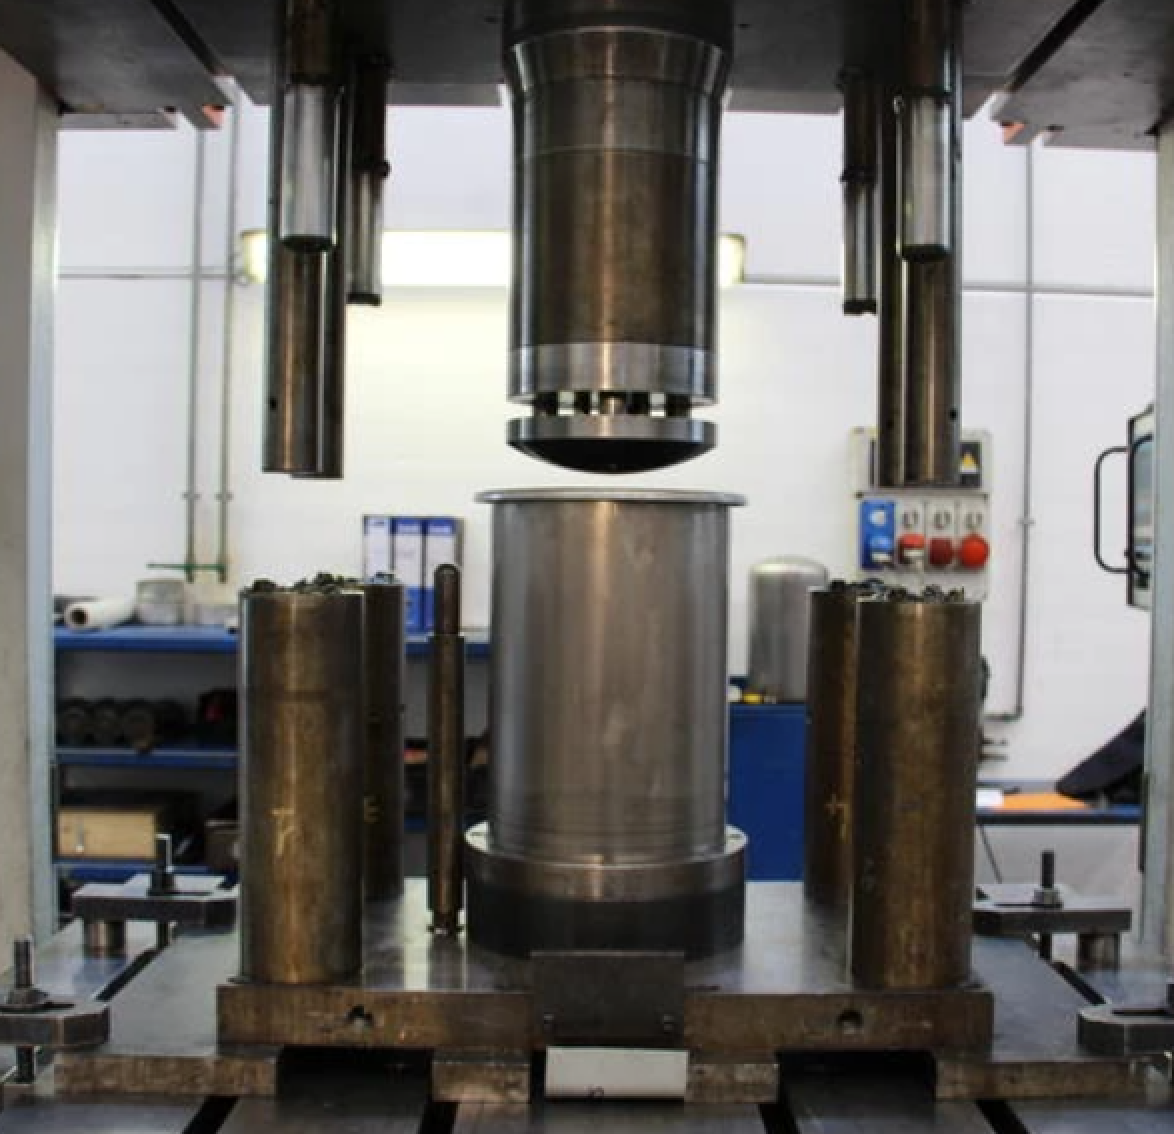
\includegraphics[scale=0.2]{Immagini/Imbutitura1.png}
    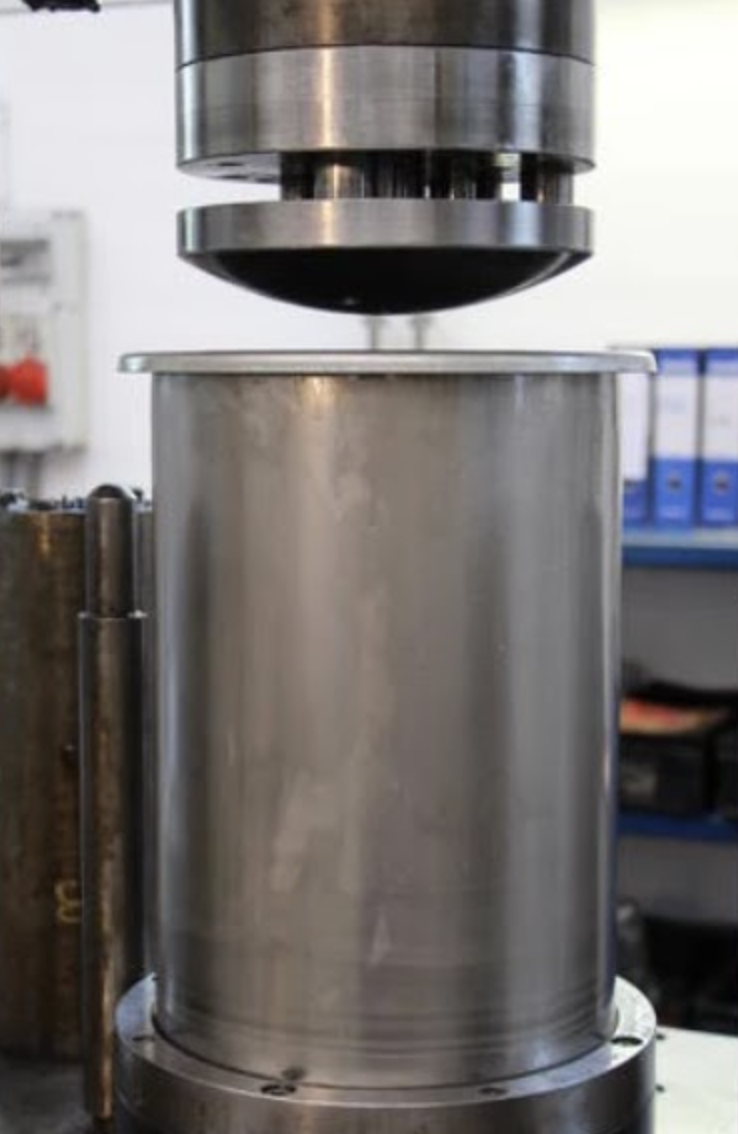
\includegraphics[scale=0.2]{Immagini/Imbutitura2.png}
    \caption{Processo produttivo di imbutitura}
    \label{fig:Imbutitura}
\end{figure}
\paragraph{Saldatura} La Saldatura ad arco sommerso è un procedimento di saldatura ad arco a filo continuo sotto protezione di scoria. La morfologia generale della zona di saldatura (cioè il fatto che l'arco scocchi sotto la scoria) permette di generare una grande quantità di calore che, essendo schermato dalla scoria, cattiva conduttrice termica, resta localizzato nel bagno di saldatura. Quindi la saldatura ad arco sommerso permette di operare con elevate velocità di saldatura e di deposito. La saldatura ad arco sommerso è un processo che può essere reso completamente automatico e può effettuare sia saldature longitudinali in posizione piana che saldature circonferenziali su posizionatori.
\begin{figure}[h]
    \centering
    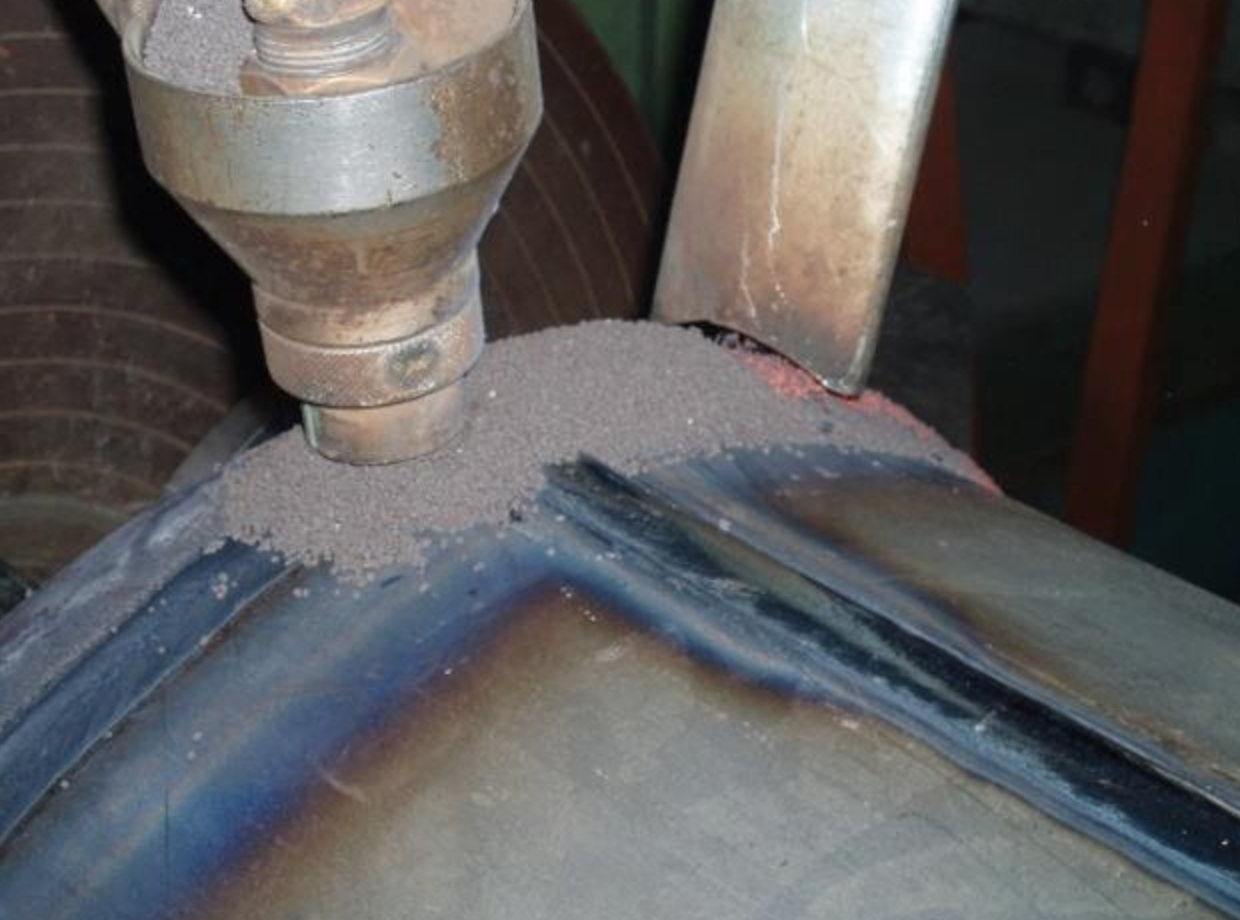
\includegraphics[scale=0.22]{Immagini/Saldatura1.png}
    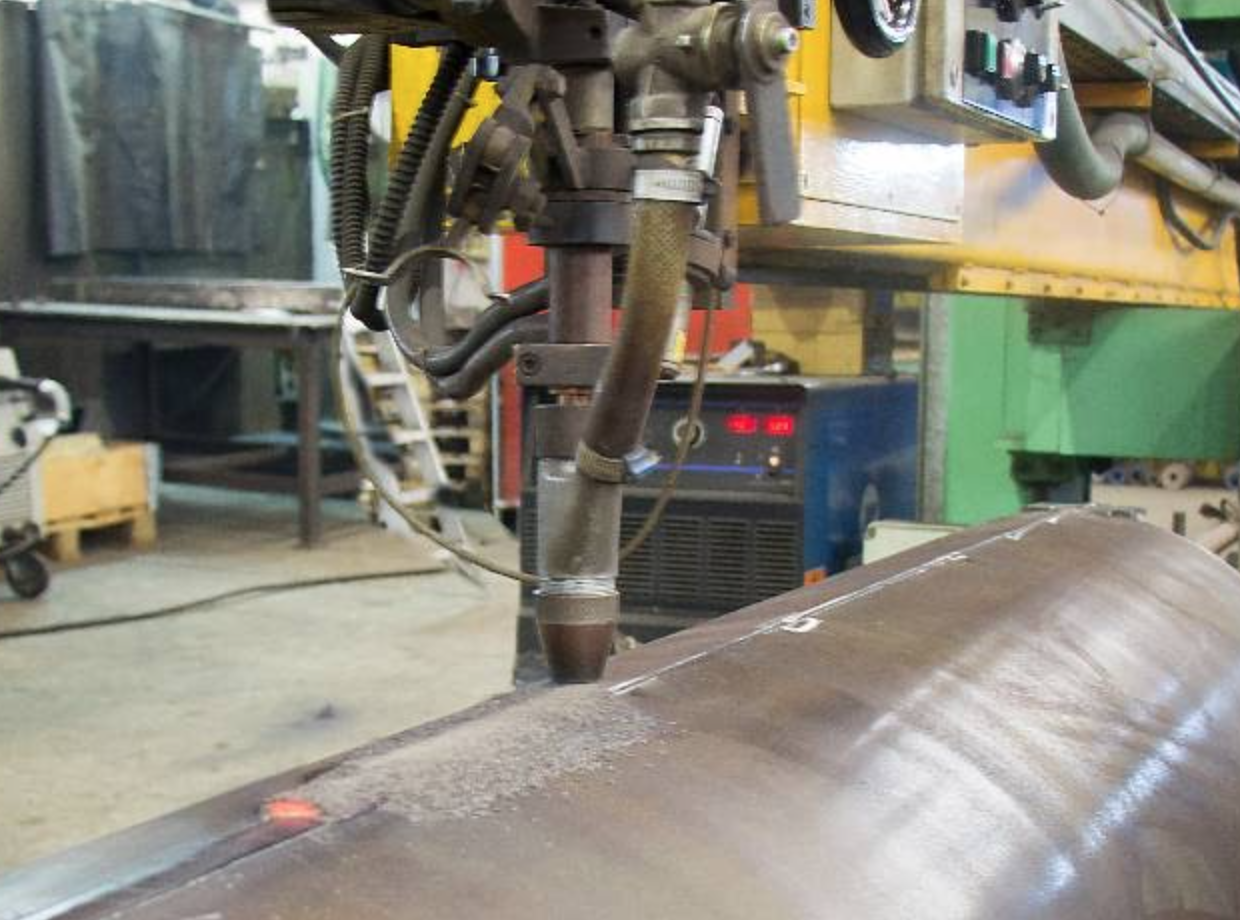
\includegraphics[scale=0.22]{Immagini/Saldatura2.png}
    \caption{Processo produttivo di saldatura}
    \label{fig:Saldatura}
\end{figure}
\paragraph{Foratura}La foratura è una lavorazione per asportazione truciolo che permette di realizzare fori mediante l’utilizzo di un utensile rotante e traslante in direzione assiale. 
\begin{figure}[h]
    \centering
    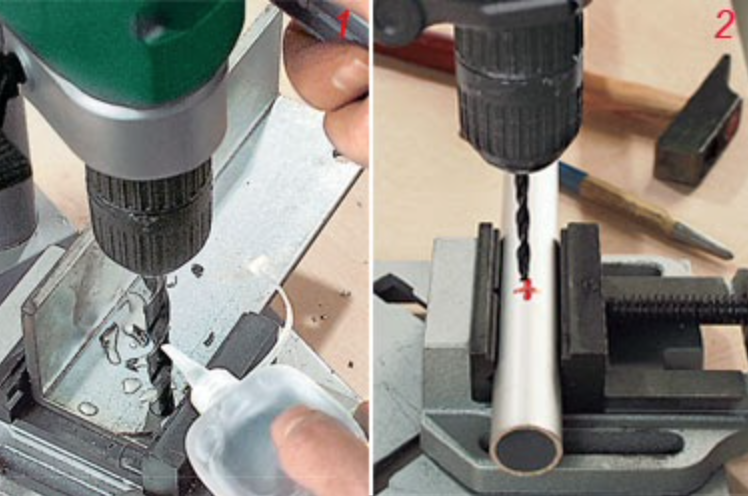
\includegraphics[scale=0.5]{Immagini/Foratura.png}
    \caption{Processo produttivo di foratura}
    \label{fig:Foratura}
\end{figure}

Segue poi la realizzazione di bocchelli per il collegamento di elementi esterni al serbatoio. Esistono differenti soluzioni tecnologiche per l'accoppiamento tra questi ultimi e i relativi fori realizzati.\\
Nel caso in analisi, essendo la pressione all'interno del serbatoio relativamente modesta, sarà sufficiente realizzare una saldatura ad angolo circonferenziale. 
\begin{figure}[h]
    \centering
    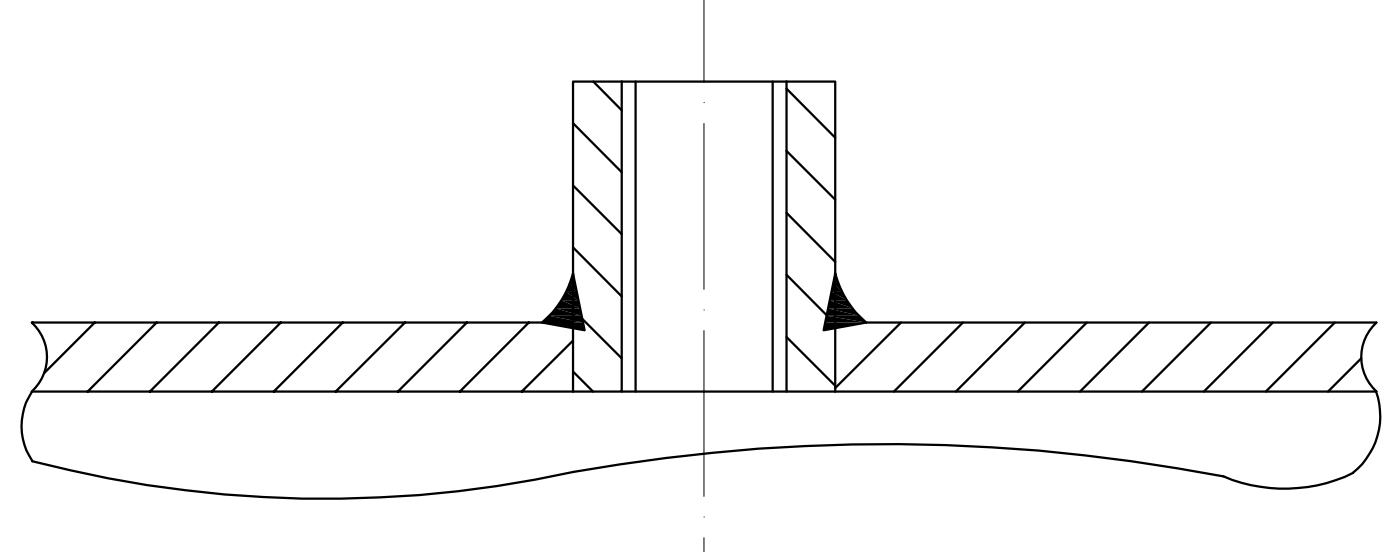
\includegraphics[scale=0.4]{Immagini/Bocchello.png}
    \caption{Sezione accoppiamento bocchello-foro}
    \label{fig:Bocchello}
\end{figure}
\subsection{Verifica resistenza del serbatoio}
Nella fase di progettazione di un serbatoio in pressione si possono seguire tre differenti metodologie:
\begin{itemize}
    \item Metodo DBF (Designed By Formula), calcolo degli spessori delle membranature mediante normative ed apposite formule ricavabili analiticamente e sperimentalmente. 
    \item Metodo DBA (Designed By Analysis), calcolo computazionale basato sul metodo agli elementi finiti (FEM).
    \item Metodo DBE (Designed By Experimenthal methods) Calcolo mediante prove tecniche sul componente (per esempio prove di scoppio). 
\end{itemize}
\paragraph{Approccio DBF} Poichè non sarebbe stato possibile utilizzare software di calcolo FEM e tanto meno realizzare prove sperimentali sul componente, si è optato di basare l'analisi e le verifiche del serbatoio sul primo approccio elencato. \\
\\
Basandosi sulla normativa VSR, sono state ricavate le formule analitiche utilizzate per la progettazione delle caratteristiche del serbatoio. \\
Per l'applicazione di tale metodo sarà necessario approssimare qualitativamente gli stati di tensione e considerare gli effetti di concentrazione degli sforzi, o di indebolimenti, mediante l'introduzione di coefficienti correttivi empirici. Si ricorda, inoltre, che questo metodo non può essere applicato per lo studio del componente a fatica.
\paragraph{Dati di progetto}
\begin{itemize}
    \item Caratteristiche meccaniche materiale: $R_m=360\ MPa$ e $R_s=235\ MPa$
    \item Caratteristiche geometriche: $D_e=370\ mm$ e $H=108\ mm$
    \item Pressione di esercizio: $p=10\ bar$
    \item Temperatura di esercizio serbatoio: $-10^{\circ}C<T<50^{\circ}C$
    \item Classe di rischio: C 3 (note $p$ e $V$, da Fig.\ref{fig:ClasseDiRischio})
\end{itemize}
\begin{figure}[h]
    \centering
    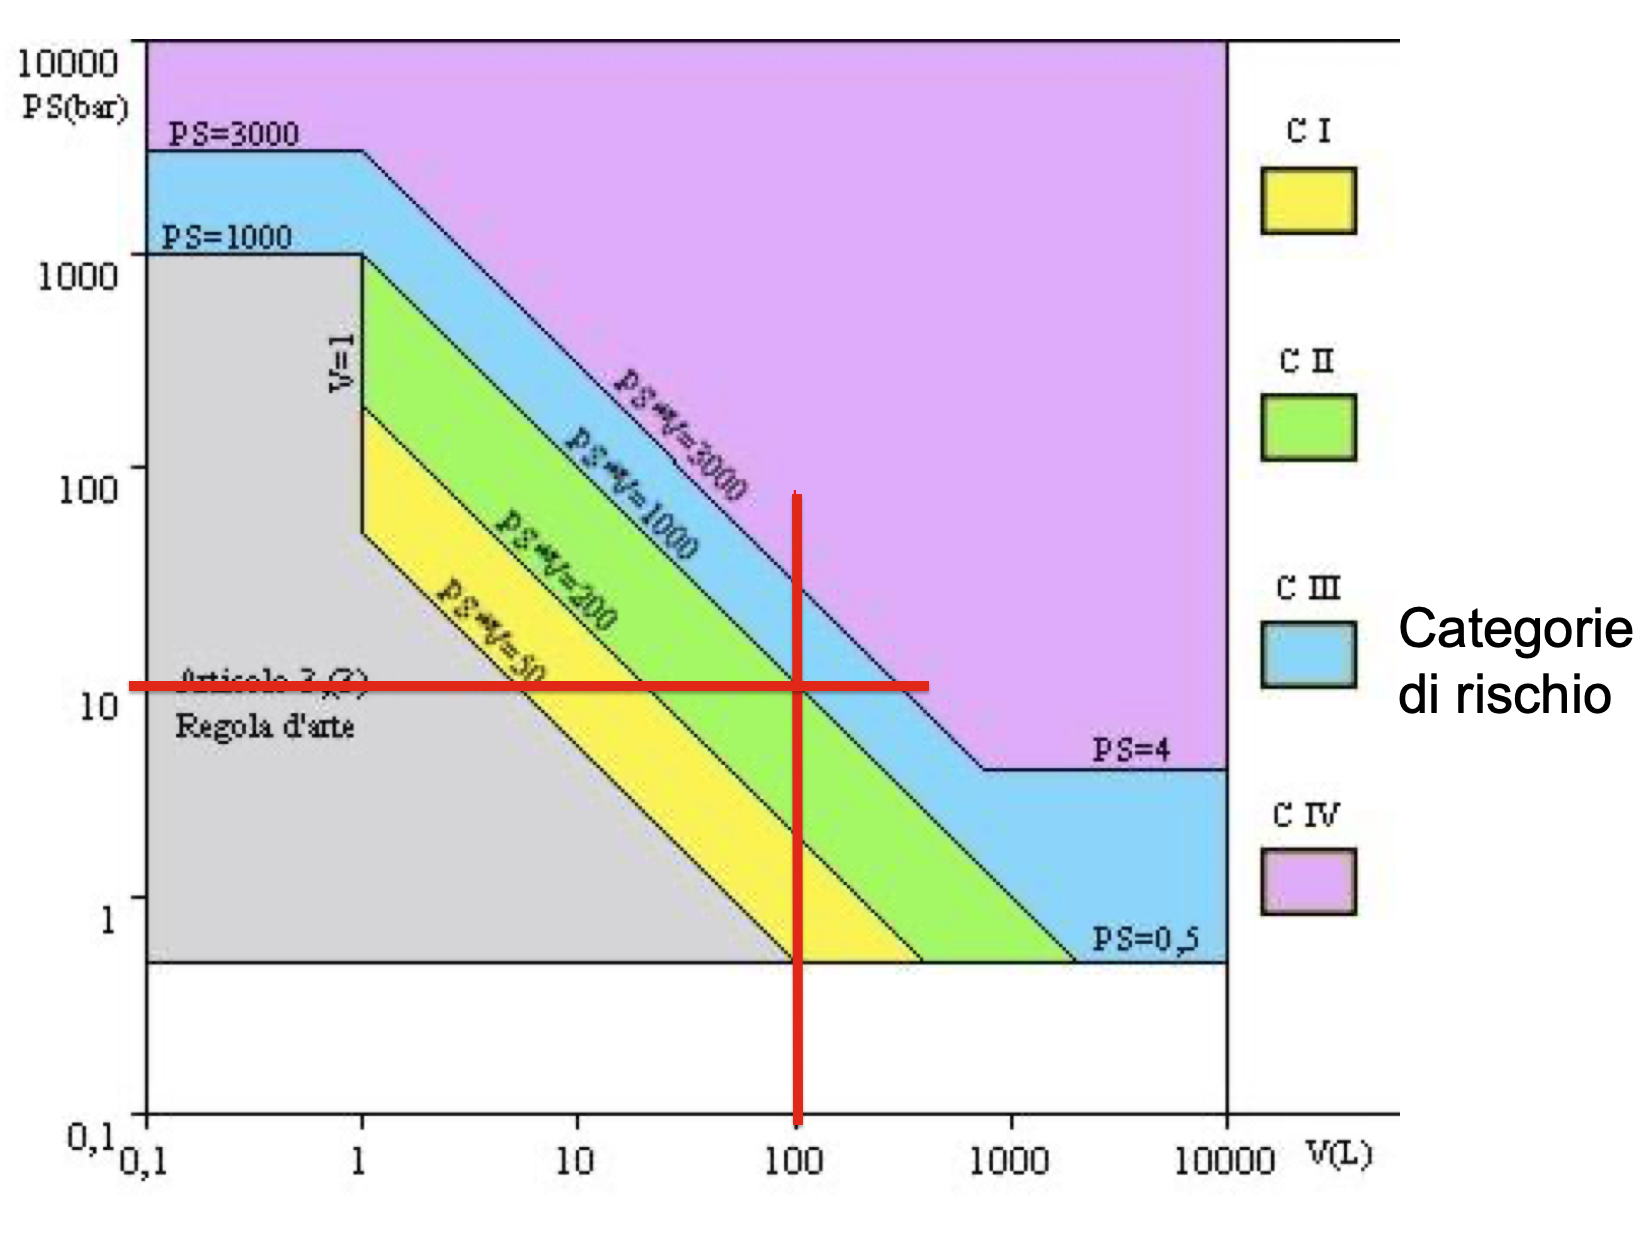
\includegraphics[scale=0.25]{Immagini/ClasseDiRischio.png}
    \caption{Classi di rischio recipienti in pressione}
    \label{fig:ClasseDiRischio}
\end{figure}
\paragraph{Massimma pressione ammissibile}
Sfruttando quanto riportato nella normativa VSR, nel paragrafo .1.b.2. , è possibile determinare la sollecitazione massima ammissibile agente sulle pareti del serbatoio in condizioni di progetto.\\
Per temperature di esercizio considerate nei dati, la massima sollecitazione è valutabile come:
\begin{equation}
    f_{Max}=min\left[\frac{R_s}{1,5};\frac{R_m}{2,4}\right]=min[157\ MPa;150\ MPa]
\end{equation}
quindi la sollecitazione massima ammissibile sarà pari a 150 MPa.
\paragraph{Minimi spessori ammissibili}
Il paragrafo .1.c.1. della stessa normativa consente di definire lo spessore minimo ammesso per serbatoi pressurizzati in funzione del processo produttivo e della tipologia di materiale con cui sono ricavati.\\
Nel caso in esame, avendo supposto come materiale l'acciao al carbonio Fe360, proveniente da processi di deformazione plastica, lo spessore risulta:
\begin{equation}
    s_{min}=3\ mm
\end{equation}
Per il tratto cilindrico, viene posta attenzione particolare nel paragrafo .1.d.2., il quale riporta come poter stimare, in condizioni di verifica, il minimo spessore di questo tratto attraverso la relazione:
\begin{equation}
    s_{0,cil}=\frac{p\cdot D_e}{\left(2\cdot f_{Max}\cdot z\right)+p}=1,23\ mm
\end{equation}
supponendo il modulo di efficienza $z=1$. \\
\\
Per i fondi, lo stesso procedimento viene considerato nel paragrafo .1.e.2., il quale riporta come poter stimare, in condizioni di verifica, il minimo spessore dei due componenti, in funzione della loro geometria attraverso la relazione:
\begin{equation}
    s_{0,fon}=\frac{p\cdot D_e}{2\cdot f_{max}\cdot z}\cdot C_0=1,09\ mm
\end{equation}
con coefficiente di forma $C_0=0,89$, ricavabile dalla retta inferiore del diagramma in Fig.\ref{fig:GraficoC0} in funzione del rapporto $H/D_e=0,292$. \\
\\
In conclusione, essendo entrambi gli spessori inferiori a quello considerato in prima analisi, si sceglie di assumere uno spessore omogeneo per il serbatoio pari a 3 mm.
\newpage
\begin{figure}[h]
    \centering
    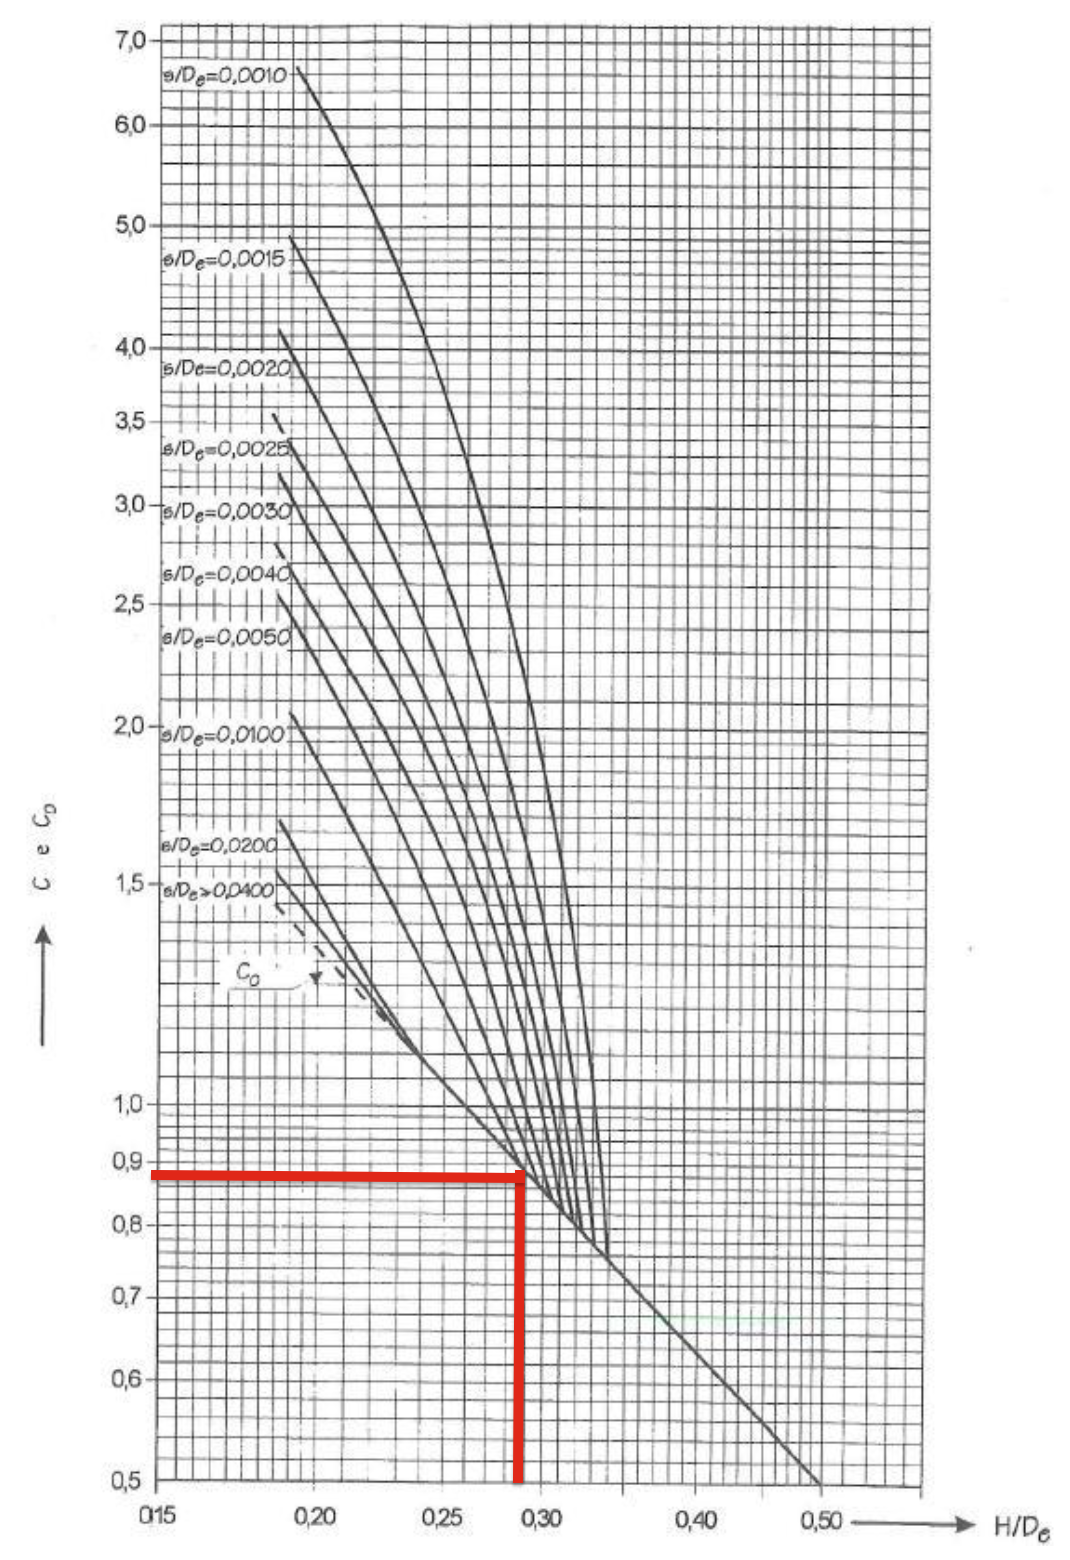
\includegraphics[scale=0.5]{Immagini/GraficoC0.png}
    \caption{Grafico per la scelta del coefficiente di forma $C_0$}
    \label{fig:GraficoC0}
\end{figure}
\subsubsection{Verifica saldature}
I recipienti in pressione vengono divisi in due categorie: quelli di piccolo spessore e quelli di grande spessore. 
Siccome lo spessore di 3 mm è relativamente piccolo, nel calcolo delle tensioni assiali, circonferenziali e radiali, si può assumere $\sigma_r=0$.
\paragraph{Cordone tratto cilindrico}
Nel tratto cilindrico agisce una tensione circonferenziale, cioè perpendicolare all'asse del cordone di saldatura, pari a:
\begin{equation}
    \sigma_{\theta}=\sigma_{\perp}=\frac{p D_e}{2t}=61,7\ MPa
\end{equation}
e una tensione assiale, cioè parallela all'asse del cordone di saldatura, pari a:
\begin{equation}
    \sigma_a=\sigma_{\parallel}=\frac{pD_e}{2\cdot 2t}=30,8\ MPa.
\end{equation}
La tensione equivalente agente sul cordone di saldatura sarà quindi pari a:
\begin{equation}
    \sigma_{eq}=\sqrt{\sigma_{\perp}^2+\sigma_{\parallel}^2-\sigma_{\perp}\sigma_{\parallel}}=53\ MPa. 
\end{equation}
La tensione equivalente calcolata dovrà risultare minore o uguale alla tensione ammissibile ricavata da Fig.\ref{fig:TensioneAmmissibileCordone} :
\begin{equation}
    \sigma{eq}\le \frac{0,85\sigma_{adm}}{n}\to n=2,6
\end{equation}
considerando un cordone di classe II.
\begin{figure}[h]
    \centering
    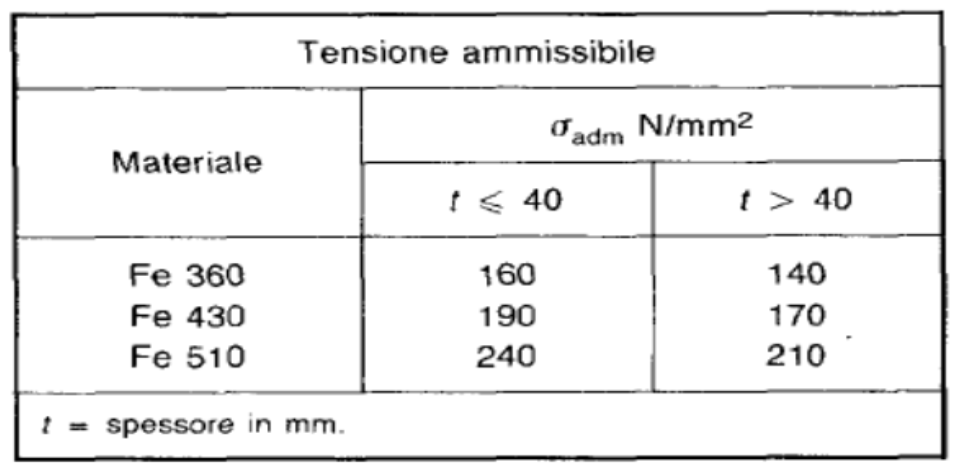
\includegraphics[scale=0.473]{Immagini/TensioneAmmissibileCordone1.png}
    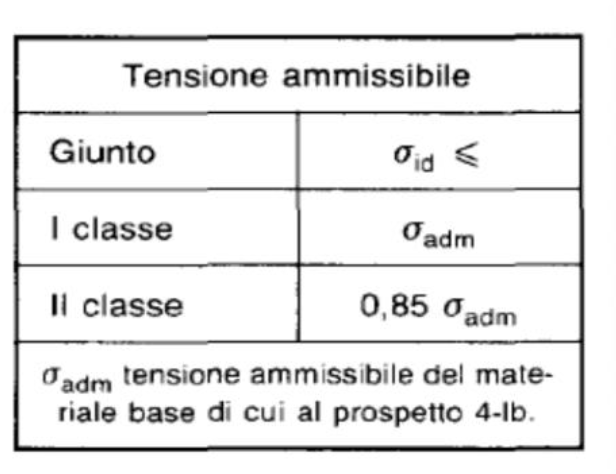
\includegraphics[scale=0.5]{Immagini/TensioneAmmissibileCordone2.png}
    \caption{Tabelle per la scelta della tensione ammissibile}
    \label{fig:TensioneAmmissibileCordone}
\end{figure}
\paragraph{Cordone fondi}
In prima approssimazione si utilizzerà un approccio analogo a quello utilizzato per la geometria dei fondi sferici, supponendo però coefficienti correttivi che adatteranno le tensioni calcolate a quelli di geometria semiellittica. \\
Nel fondo agisce una tensione circonferenziale pari a :
\begin{equation}
    \sigma_{\theta}=\frac{pD_e}{2\cdot 2t}=30,8\ MPa
\end{equation}
e una tensione assiale di uguale valore, essendo la geometria sferica. 
Poichè nel fondo semiellittico la tensione assiale sarà maggiore rispetto a quella circonferenziale, considereremo i seguenti fattori correttivi:
\begin{itemize}
    \item $\sigma_a=\sigma_a\cdot 1,5=46,2\ MPa$.
    \item $\sigma_{\theta}=\sigma_{\theta}\cdot 0,5=15,4\ MPa$,
\end{itemize}
La tensione equivalente agente sul cordone di saldatura sarà pari a:
\begin{equation}
    \sigma_{eq}=\sqrt{\sigma_{\perp}^2+\sigma_{\parallel}^2-\sigma_{\perp}\sigma_{\parallel}}=40,7\ MPa. 
\end{equation}
La tensione equivalente calcolata dovrà risultare minore o uguale alla tensione ammissibile ricavata da Fig.\ref{fig:TensioneAmmissibileCordone} :
\begin{equation}
    \sigma{eq}\le \frac{0,85\sigma_{adm}}{n}\to n=3,3
\end{equation}
considerando un cordone di classe II.\\
\\
I cordoni di saldatura risultano quindi verificati.